\chapter{Results and Discussion}

\section{Sequence Comparison using Multiple Sequence Alignment}

The first step of our methodology is to study the similarities and differences in the amino-acid sequences of the ensemble of GSTs that we are interedt in (25 sequences). It will provide us the global information about how well-conserved is this ensemble of structures. To do so, we used the Multiple Sequence Alignment (MSA) tool as presented in the section 2.1. From MSA, we computed the percentage of identity between pairs of sequences. This score corresponds to the amount of amino acids that are identical between two sequences. As shown in Fig.~\ref{Sequence and Structure matricies}a, the percentage of identity between GSTs belonging to the class $\delta$ is relatively high, with values ranging between 50 and 80\% identity. In addition, if we except the case of the GSTD11 which presents a singular behavior compared to the other GSTs from class $\delta$, the percentage identity is always larger than 60\%.

For the class $\varepsilon$, the results are slightly different. Except for GSTs E5, E6, E7, E8 that show relatively high percentage identity within each others (around 70\%, Fig.~\ref{Sequence and Structure matricies}a), the overall sequence identity score between GSTs from the class $\varepsilon$ is lower (around 40-50\%). Particularly, the GSTE14 presents a singular behavior with identity score between 20-30\%. Moreover, the comparison between the two classes $\delta$ and $\varepsilon$ shows that the sequence identity is . It means that even though GSTs are from the same organism (\textit{i.e. Drosophilia Melanogaster}), the differences of sequences between two distinct classes are non negligible. Finally, we computed the histogram of percentage identity for the ensemble of the 25 GST structures. As shown in Fig.~\ref{Sequence and Structure matricies}b, the most probable identity score range for the ensemble of 25 GSTs studied in the present work is $[-]$\%. 

\begin{figure}[h!]
	\label{Sequence and Structure matricies}
	\begin{minipage}{.48\linewidth}
		\textbf{(a)}\\
		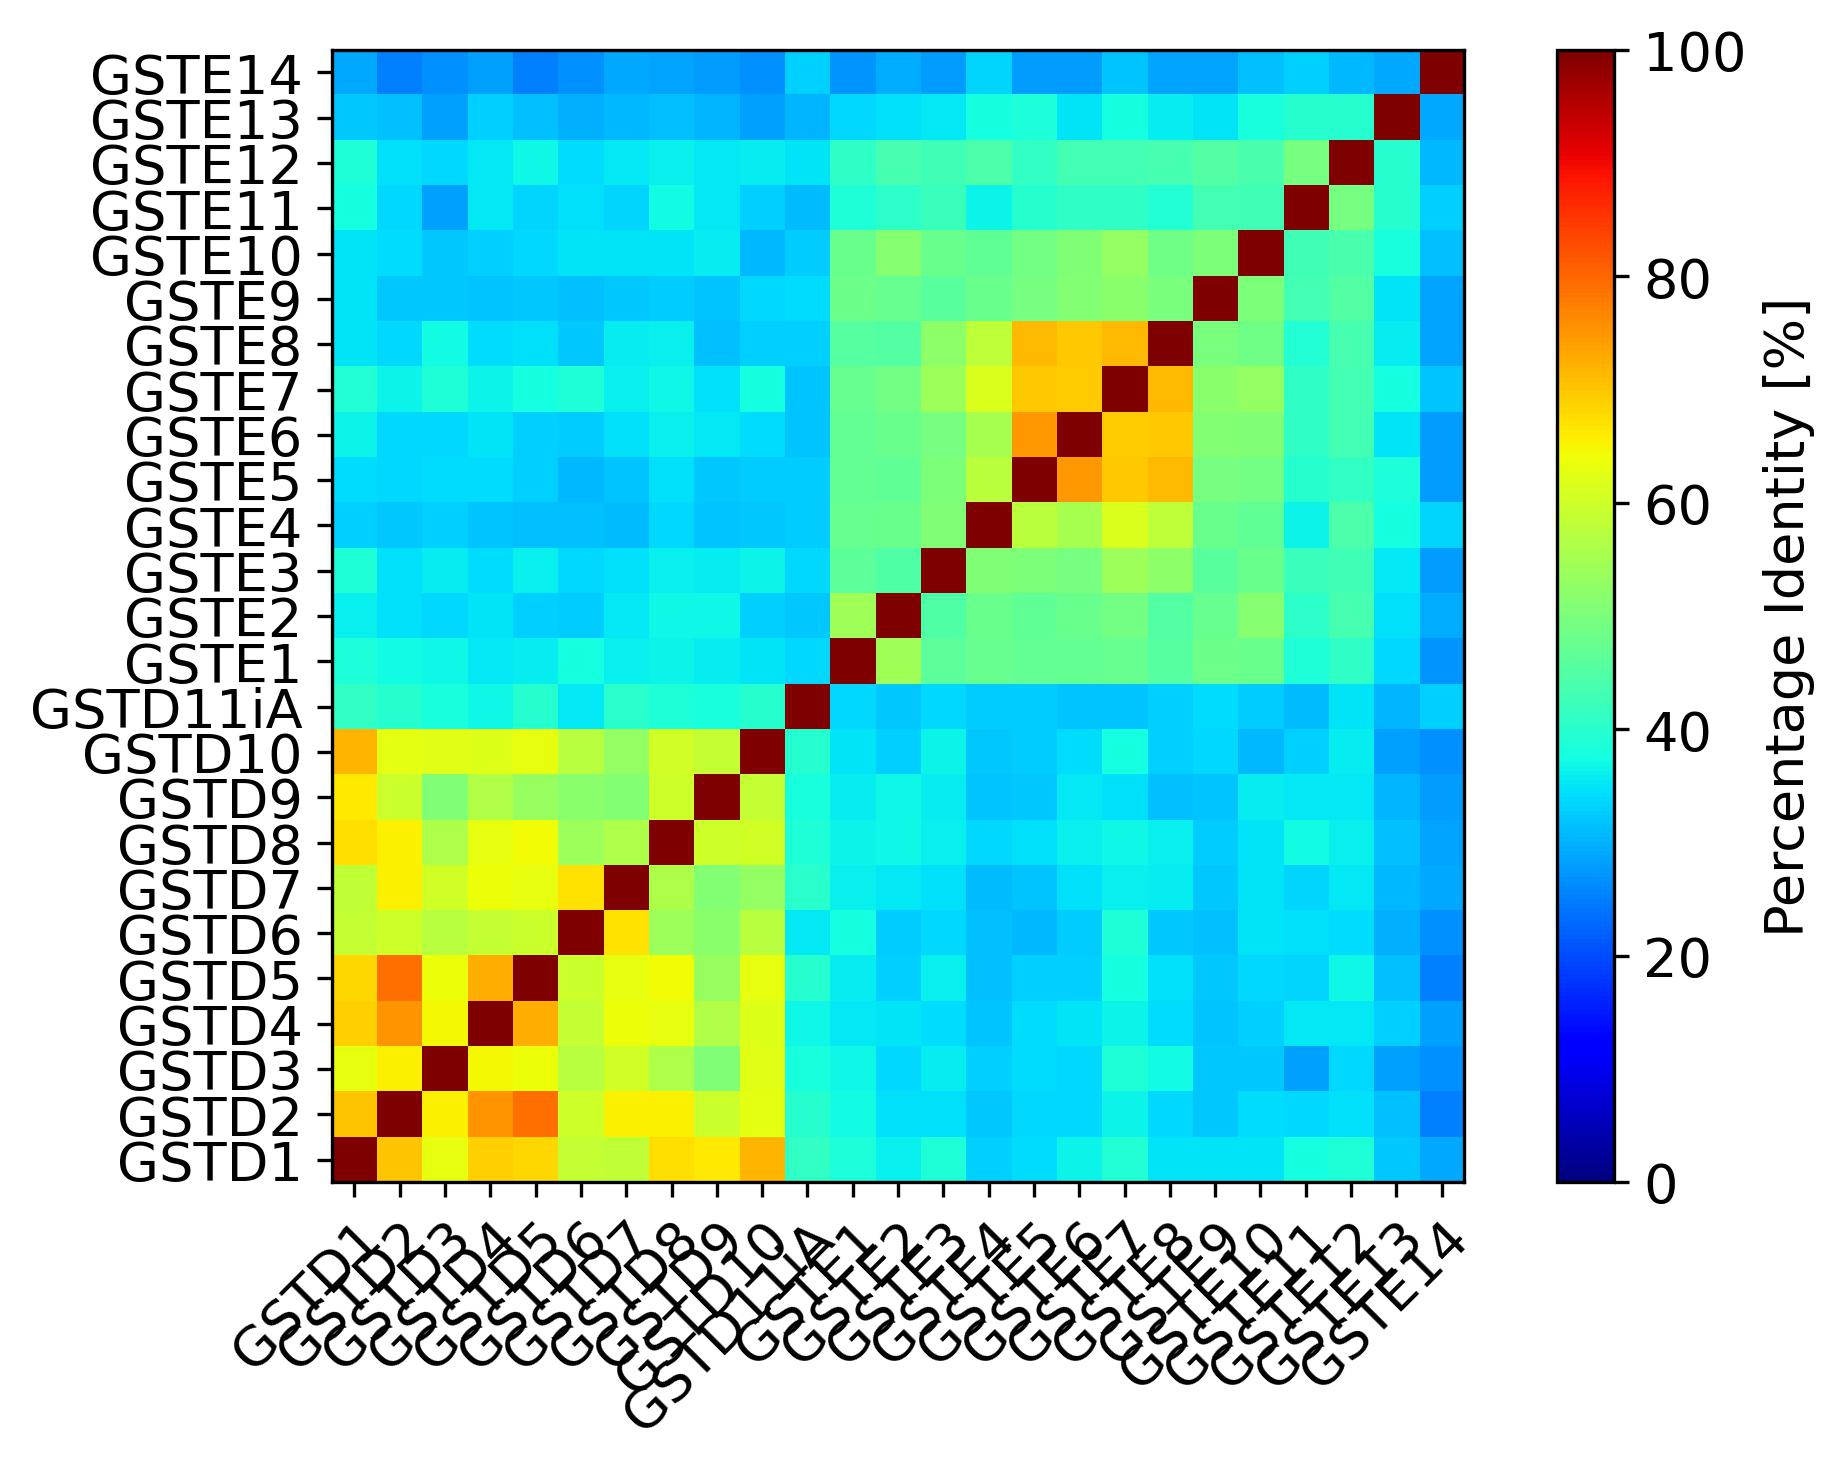
\includegraphics[height = 6cm]{figures/PercentID_matrix.jpg}
	\end{minipage}
	\begin{minipage}{.48\linewidth}
		\textbf{(b)}\\
		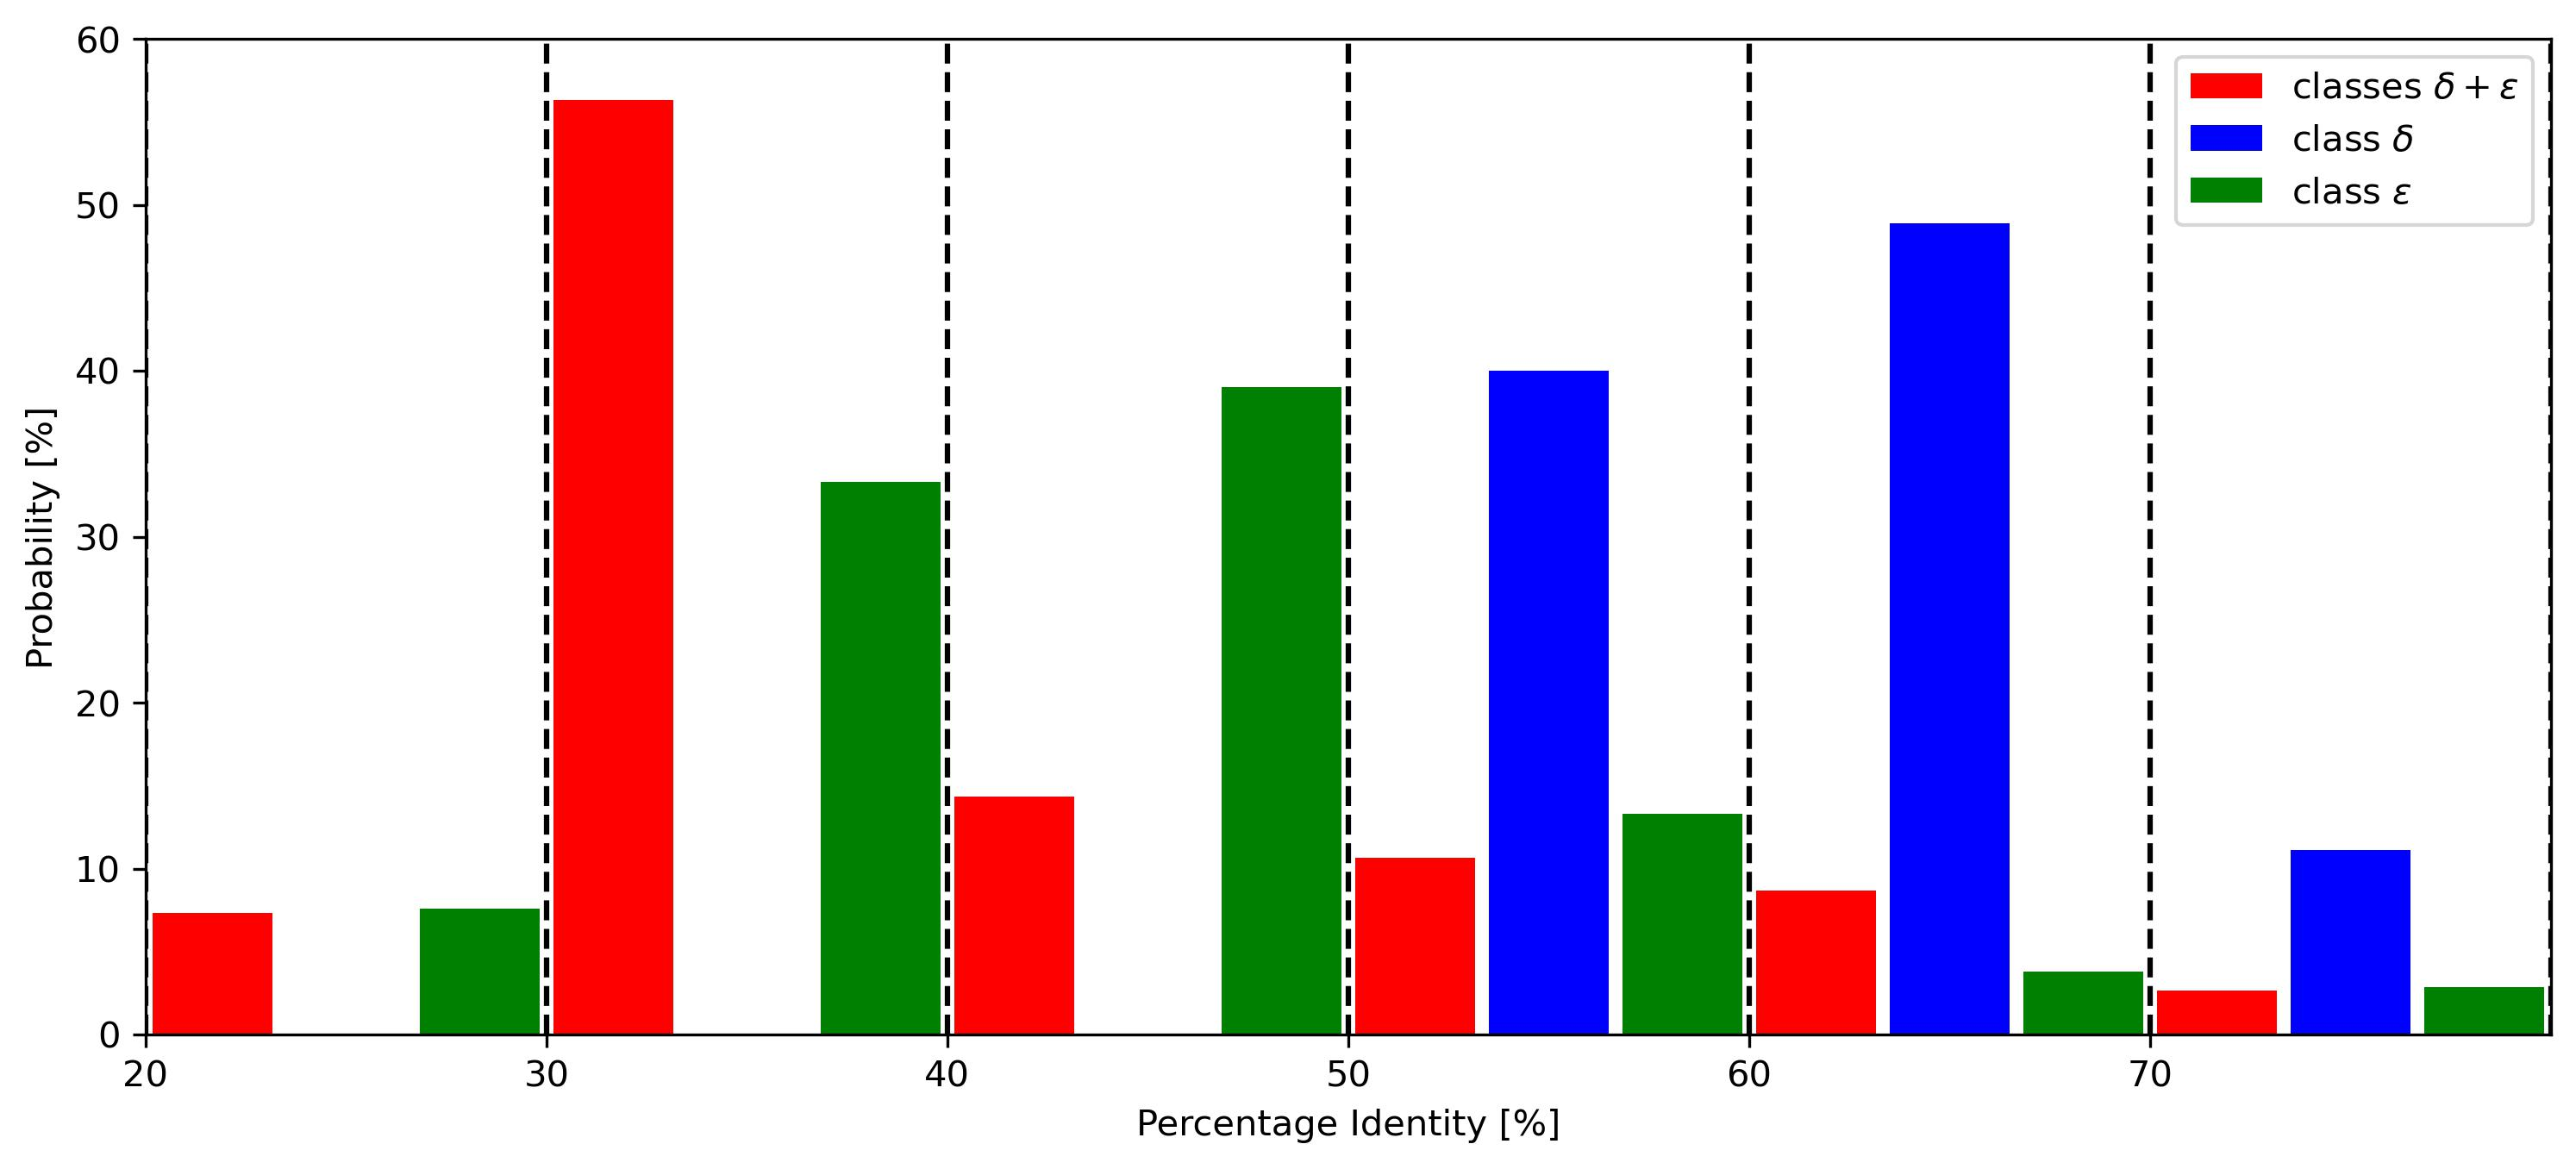
\includegraphics[height = 5.5cm]{figures/PercentID_proba.jpg}
		\vspace{.15cm}
	\end{minipage}
	\caption{a) Percentage identity matrix ($25\times 25$) computed between each pair of sequences. b) Histogram of Percentage identity scores. Blue, green and red bars indicate classes $\delta$; $\varepsilon$ and both $\delta+\varepsilon$, respectively.}
\end{figure}

\section{Structures of GSTs Predicted by AI}

\subsection{Prediction of APO (unbound) structures using AlphaFold}

Fig.~\ref{AlphaFold structures} present the 25 static APO structures generated from AlphaFold2. Visually, it is not very obvious to localize the differences because the overall shape/folding of the protein is very similar. We can only point out some local conformation differences for GSTE10 and E14 at the C-terminal parts. It comes mainly from the fact that GSTE10 and E14 are the ones with the longest amino-acid sequence among the ensemble of 25 GSTs. Moreover, in order to characterize and quantify the structural ensemble obtained from AlphaFold2, each pair of GST structures were aligned and compared together by computing the Root Mean Squared Deviation metric, \textit{i.e.} the average of the geometrical distances between atoms, as shown in Fig.~\ref{AlphaFill & GSHs}a. This was done using the program PyMOL (\bulurl{https://pymol.org/}).

\begin{figure}[h!]
	\centering
	\label{AlphaFold structures}
 	\includegraphics[width = \linewidth]{figures/GSTs_array}
	\caption{Cartoon representation of the ensemble of 25 GST structures predicted from AlphaFold. The color code is: from N-terminal (red) to C-terminal (blue).}
\end{figure}

From RMSD matrix shown in Fig.~\ref{}, we identify two main clusters, one for class $\delta$ and one for $\varepsilon$, as observed for the sequence comparison. However the GSTE10 structure is characterized by higher RMSD values than the other GST structures, particularly when compared to GSTD3. In fact, it is due to the fact that GSTE10 has a longer amino acid sequence (see Fig.~\ref{}) located in the C-terminal part with an extra $\alpha$-helix. In the case of the GSTE14, the C-terminal part is unfolded.

\begin{figure}[h!]
	\label{AlphaFold RMSD}
	\begin{minipage}{.48\linewidth}
		\textbf{(a)}\\
		\centering
		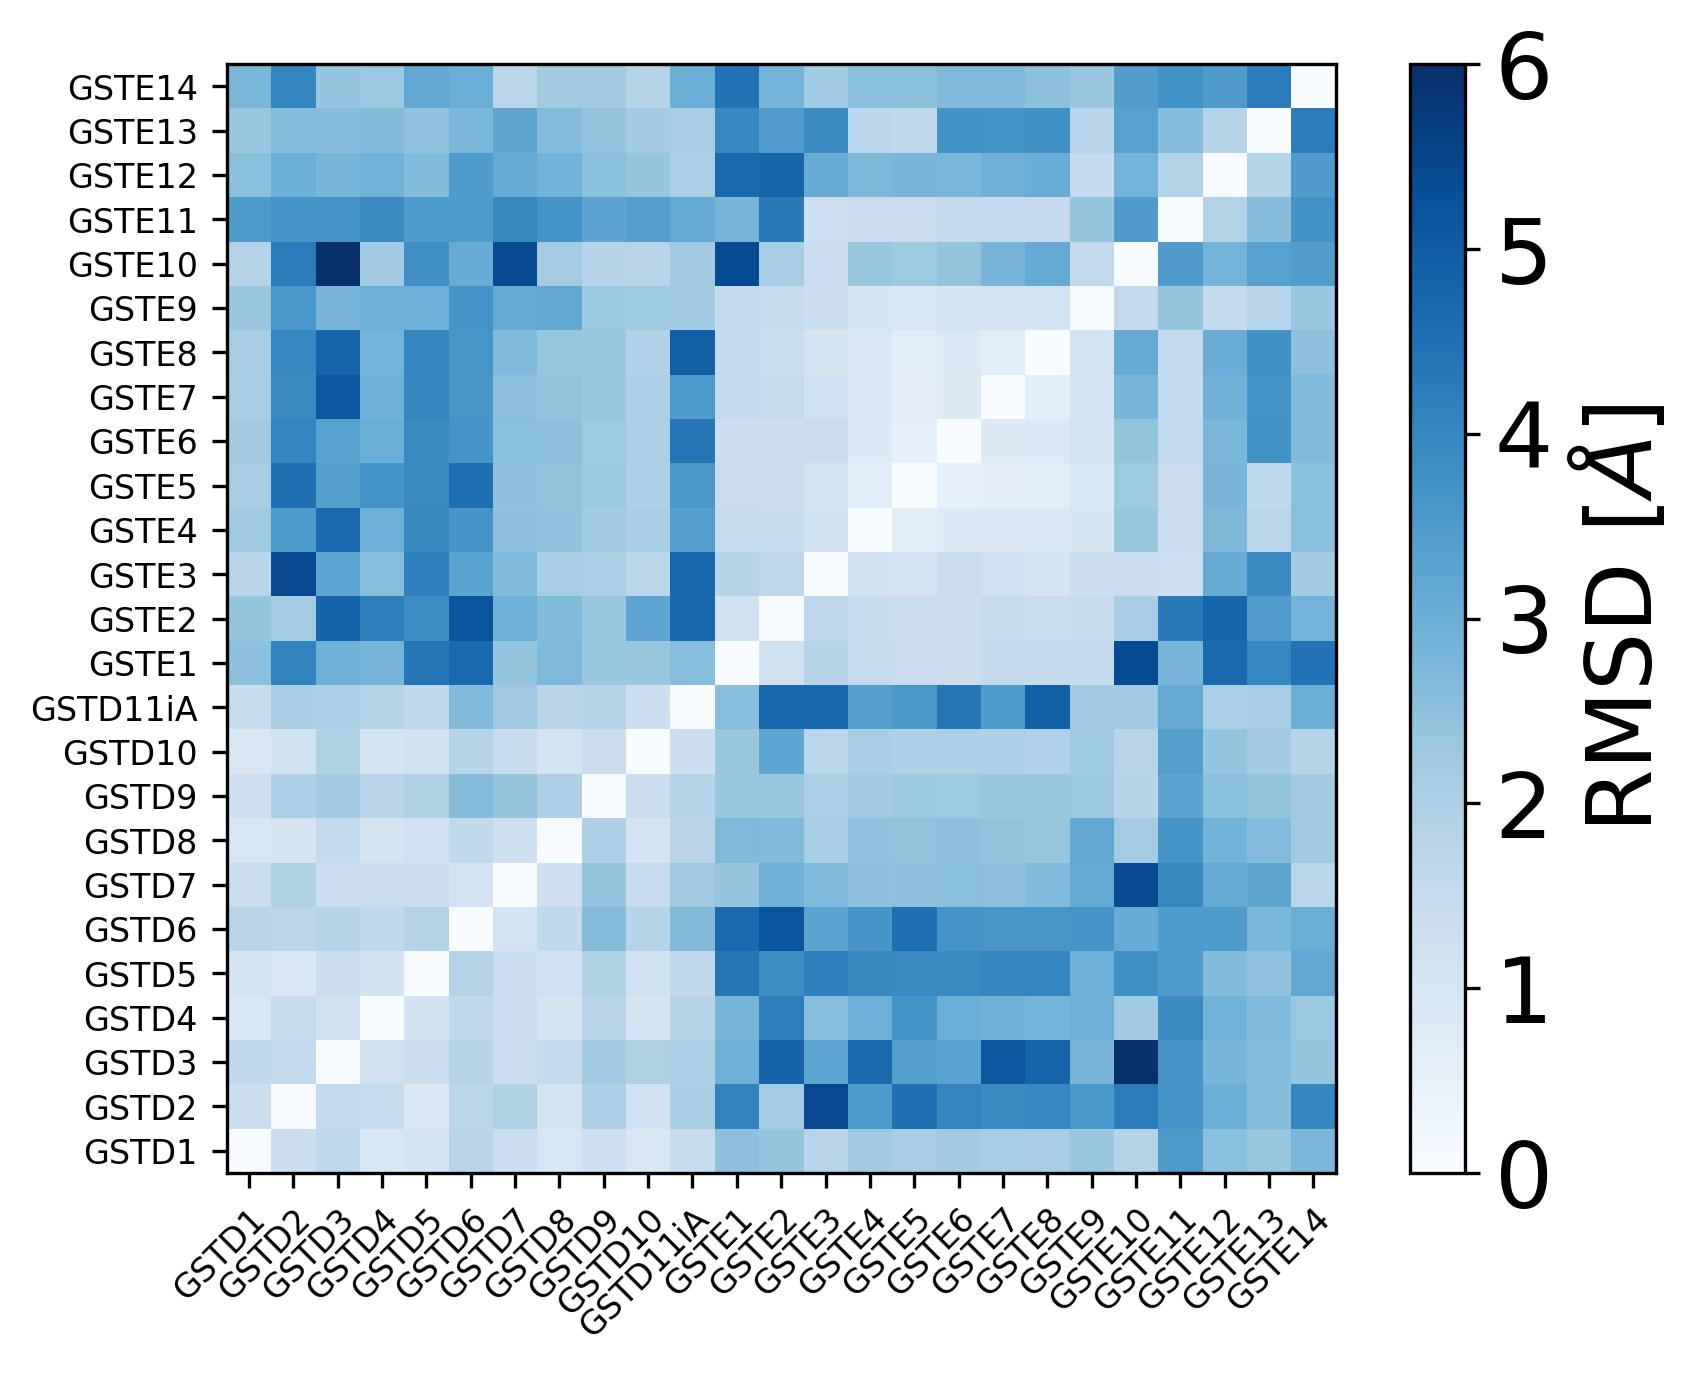
\includegraphics[height = 6cm]{figures/RMSD_matrix.jpg}
	\end{minipage}
	\begin{minipage}{.48\linewidth}
		\textbf{(b)}\\
		\centering
		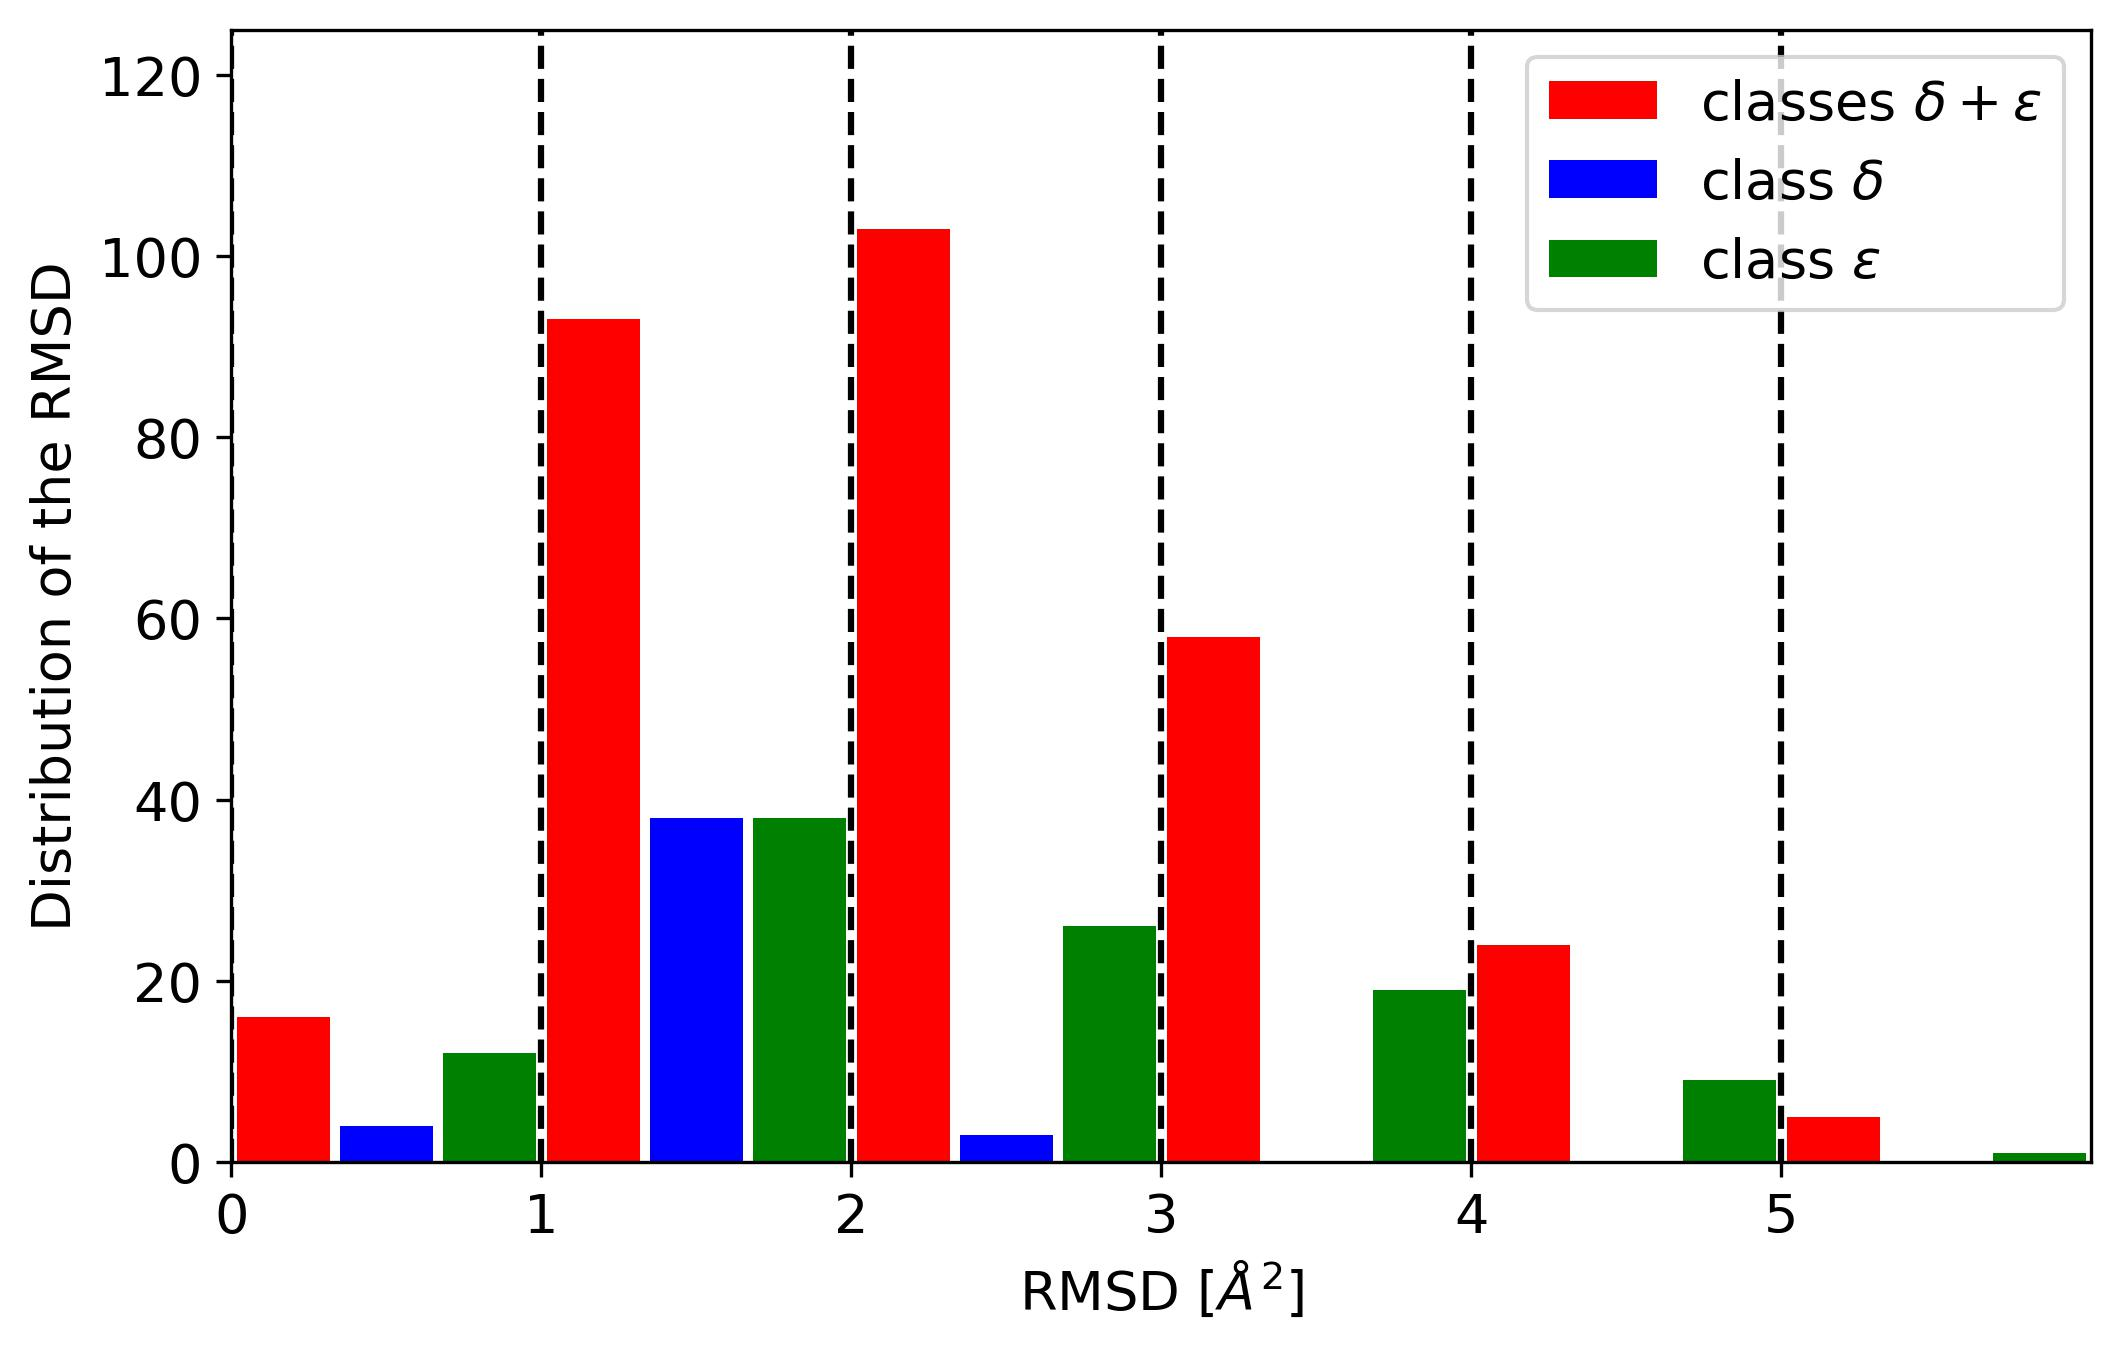
\includegraphics[height = 5.5cm]{figures/RMSD_Proba.jpg}
		\vspace{.15cm}
	\end{minipage}
	\caption{a) RMSD matrix ($25\times 25$) computed between each pair of structures. b) Histogram of RMSD scores. Blue, green and red bars indicate classes $\delta$; $\varepsilon$ and both $\delta+\varepsilon$ classes, respectively.}
\end{figure}

\subsection{Prediction of ligand positions using AlphaFill}
From the rise of AlphaFold, several tools have been developed very recently to continue the transformative effect of artificial intelligence on biomolecular sciences, for better predictions of proteins model. Indeed, the predicted protein models in the AlphaFold protein structure database, however, all lack coordinates for small molecules (\textit{i.e.} ligands), essential for molecular structure or biological functions.

AlphaFill is an algorithm based on sequence and structure similarity that "transplants" missing ligands to the AlphaFold models~\cite{AlphaFill}. For each of the 25 GST structures presented in Fig.~\ref{AlphaFold structures}, we used the AlphaFill program to predict the positions of Gluthatione ligands in GSTs. On average,AlphaFill predicts 40 different Glutathione-like ligand positions for each GST. Fig.~\ref{AlphaFill & GSHs}b shows the GSH positions predicted by AlphaFill in the case of the GSTD1. The 40 ligand positions are associated to a unique monomer but for computation purpose, we replicate the ligand positions in the second monomer as well.

Finally, as show in Fig.~\ref{}, the ensemble of ligand positions obtained from AlphaFill can be heterogeneous, with X distinguishable binding sites observed visually. All these positions will be considered as an ensemble of ligand positions for each GST and will be included in the following structural dynamics calculations.

\section{Conservation of Amino Acids in the Binding Sites and the Interface of Dimerization of GSTs}

From the atomic structures of the 25 GSTs presented in Fig.\ref{AlphaFold structures} including ligand predictions from AlphaFill and by computing contact matrices between pairs of atoms, we characterize the sequence conservation of two main structural features of GST enzymes:
\begin{itemize}
	\item the Binding Sites (BSs)
	\item the Interface of Dimerization (IoD)
\end{itemize}

Technically, two amino acids are considered to be in contact if the geometrical distance between at least the distance between one pair of heavy atoms is smaller than $3$\AA. This characteristic was computed for all the 25 GST structures and projected onto the Multiple Sequence Alignment matrix computed before (see Fig. X). In total, we identified X and Y amino acids that belongs to the BSs and IoD, respectively. It is not surprising that we found a lot of amino acids that belongs to the BSs since GSTs are well-known to recognize a large number of molecules as ligands.

Then, we computed the probability of a given amino acid to belong to the BSs or the IoD as a function of the MSA index (Fig.~\ref{BS & DI Proba}a). For each MSA index of interest, i.e. where the probability of an amino acid to belong to BSs or IoD is not negligible ($> X\%$), we computed the conservation of amino acid in the ensemble of 25 GSTs. As shown in Fig.~\ref{BS & DI Proba}c,  the amino acid with a MSA index $j=124$ and which belongs to the BSs is characterized by a high degree of conservation among the 25 GSTs  studied. For more than 40\% of the 25 sequences (mainly in the class $\delta$), the amino acid is a Tyrosine (Y, hydrophobic aromatic) whereas for the others (mainly the class $\varepsilon$), it can be a conserved substitution: a Phenylalanine (F, hydrophobic aromatic) or non-conservative ones: positively (K, R) or negatively (E) charged, polar neutral (S) or hydrophobic non-aromatic (I).\\

Add something about IoD selected MAS index (panel c)

\begin{figure}[H]
	\label{BS & DI Proba}
	\begin{minipage}{.99\textwidth}
		\textbf{(a)}\\
		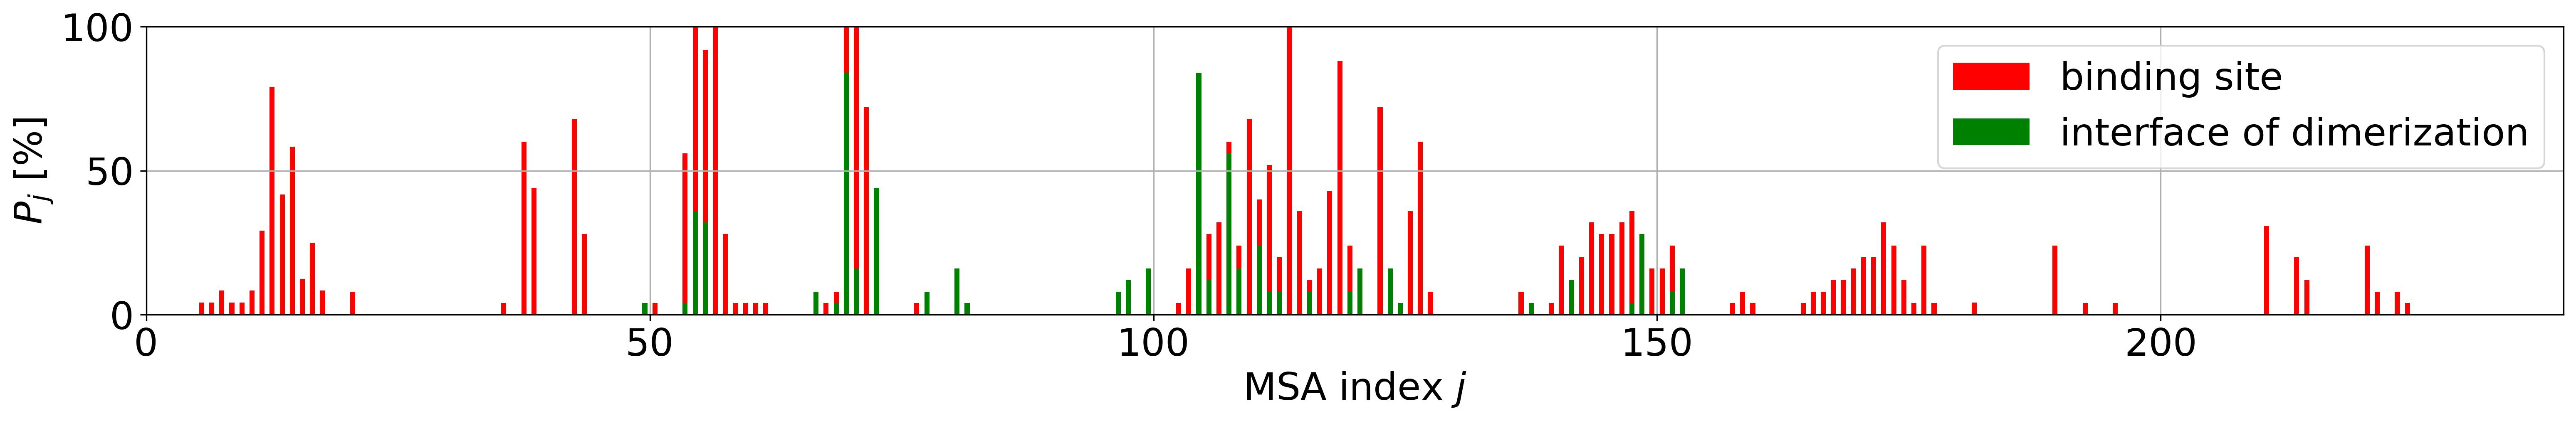
\includegraphics[width=\textwidth]{figures/MSA_Proba.jpg} % BS & DI proba
	\end{minipage}
	\begin{minipage}{.49\linewidth}
		\textbf{(b)}\\
		structure 
	\end{minipage}	
	\begin{minipage}{.48\linewidth}
		\textbf{(c)}\\
		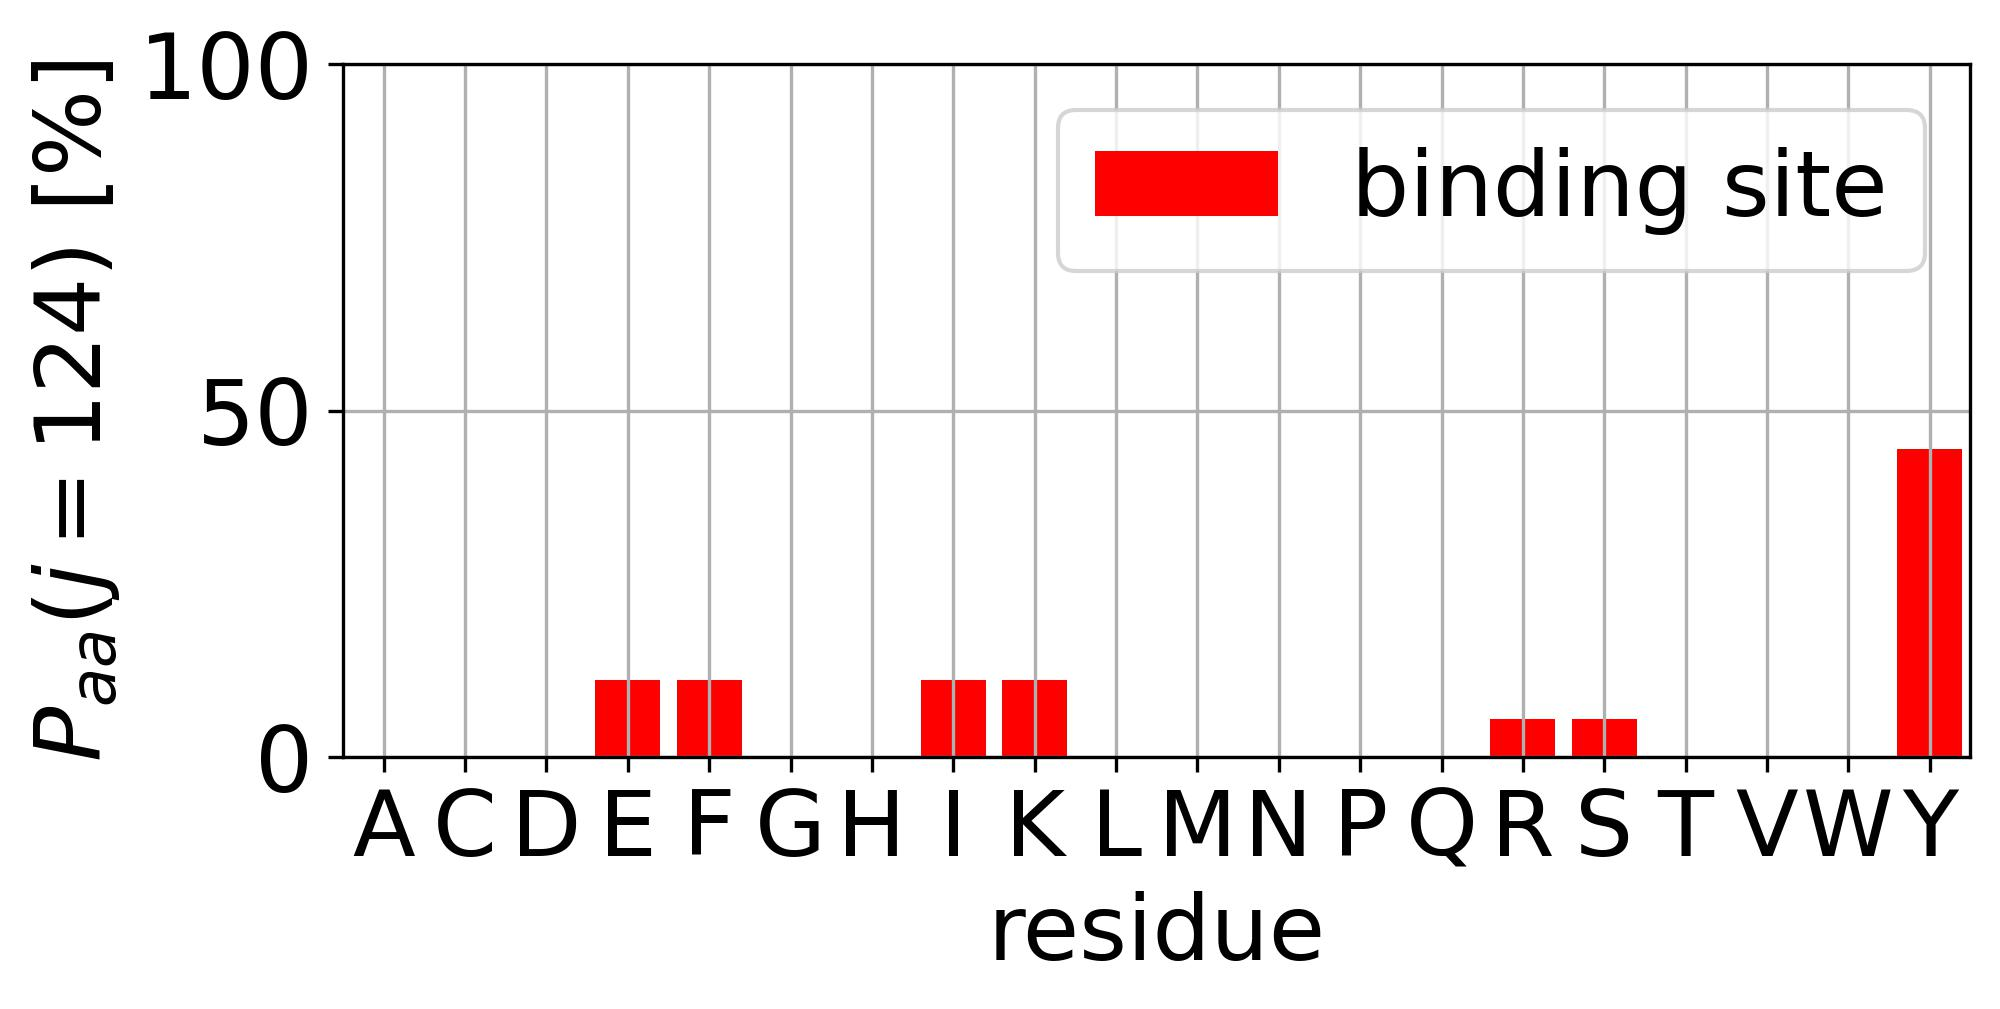
\includegraphics[width=\textwidth]{figures/amino-acid_conservation_BS_j=124.jpg}
		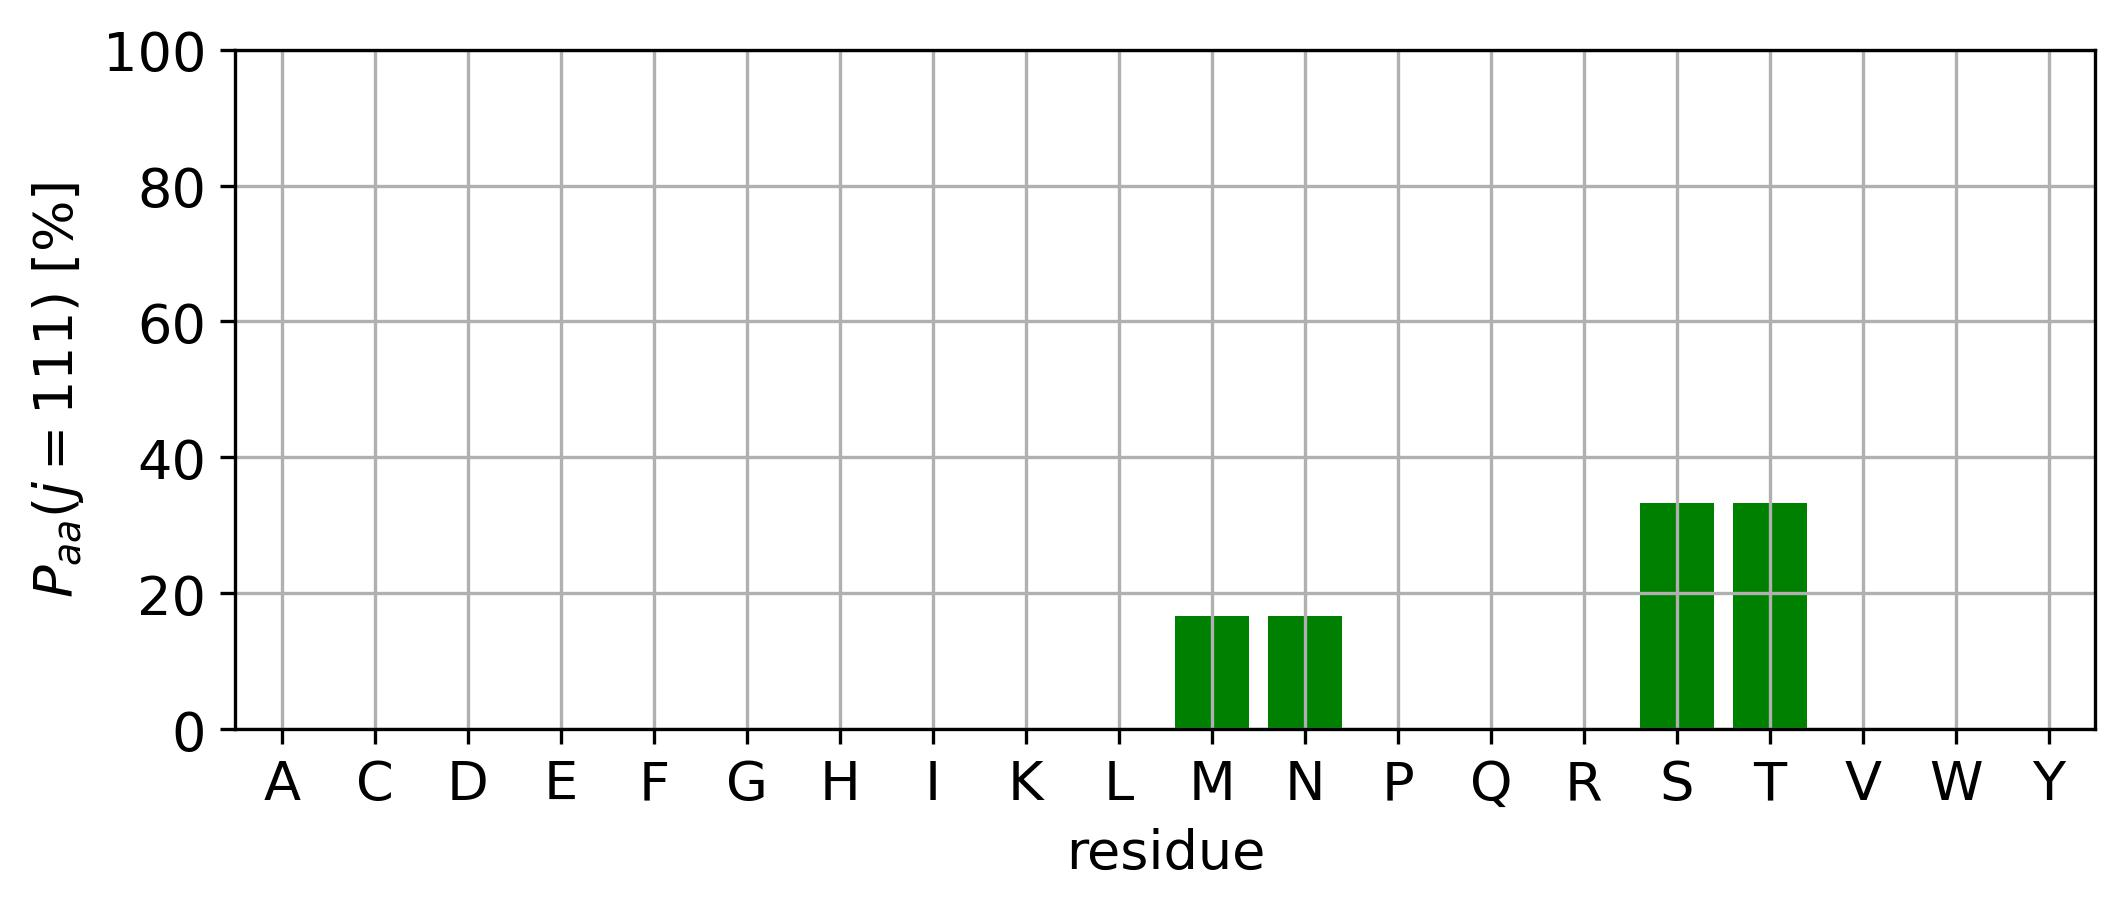
\includegraphics[width=\textwidth]{figures/amino-acid_conservation_DI_j=111.jpg}
	\end{minipage}	
	\caption{(a) Probability for an amino acid to belong to the BSs (in red) or in the IoD (in green) as a function of the MSA index. (b) Cartoon representation of the GSTD1 structure. Amino acids belonging  to the BSs (in red) and the IoD (in green) are shown in transparent spheres. (c) Probability of conservation of a given amino acid in the binding sites (top panel) and in the IoD (bottom panel).}
\end{figure}

\section{Dynamics of GSTs from Normal Mode Analysis}

From the 25 static structures of GSTs predicted from AlphaFold (Fig.~\ref{AlphaFold structures}), we first applied Normal Mode Analysis using the Anosotropic Network Model (ANM) presented in section X in order to study the local and non-local flexibility along the amino acid sequences.

\subsection{Local Mean Square Fluctuations}

Fig.~\ref{Local MSF D1} presents the computed local MSF $\sigma^2(\vv{R}_i)$ as a function of the sequence index $i$ for the GSTD1. We computed the local MSF for two structures of GSTD1: i) the APO structure, without ligand and predicted from AlphaFold and ii) the GSH structure, with GSH ligands bound to the GSTD1 predicted by AlphaFill (see section X). The goal here is to estimate the influence of the ligand to the local flexibility. As shown in Fig.~\ref{Local MSF D1}a, the presence of the ligand tends to decrease the local flexibility of two specific regions compared to the APO structure, \textit{i.e.} regions X ($\alpha_2$) and Y (loop between $\alpha_6$ and $\alpha_7$ helices).
In addition, these two regions are located very close to the BSs and the IoD (Fig.~\ref{Local MSF D1}b and c). Particularly, the flexibility of the loop between $\alpha_6$ and $\alpha_7$ helices seems to play an important role for both the BSs and the IoD since several residues are located just before or just after this region. This loop may be involved in the binding and/or releasing of the ligands.

\begin{figure}[h!]
	\begin{minipage}{\linewidth}
		\textbf{(a)}\\
		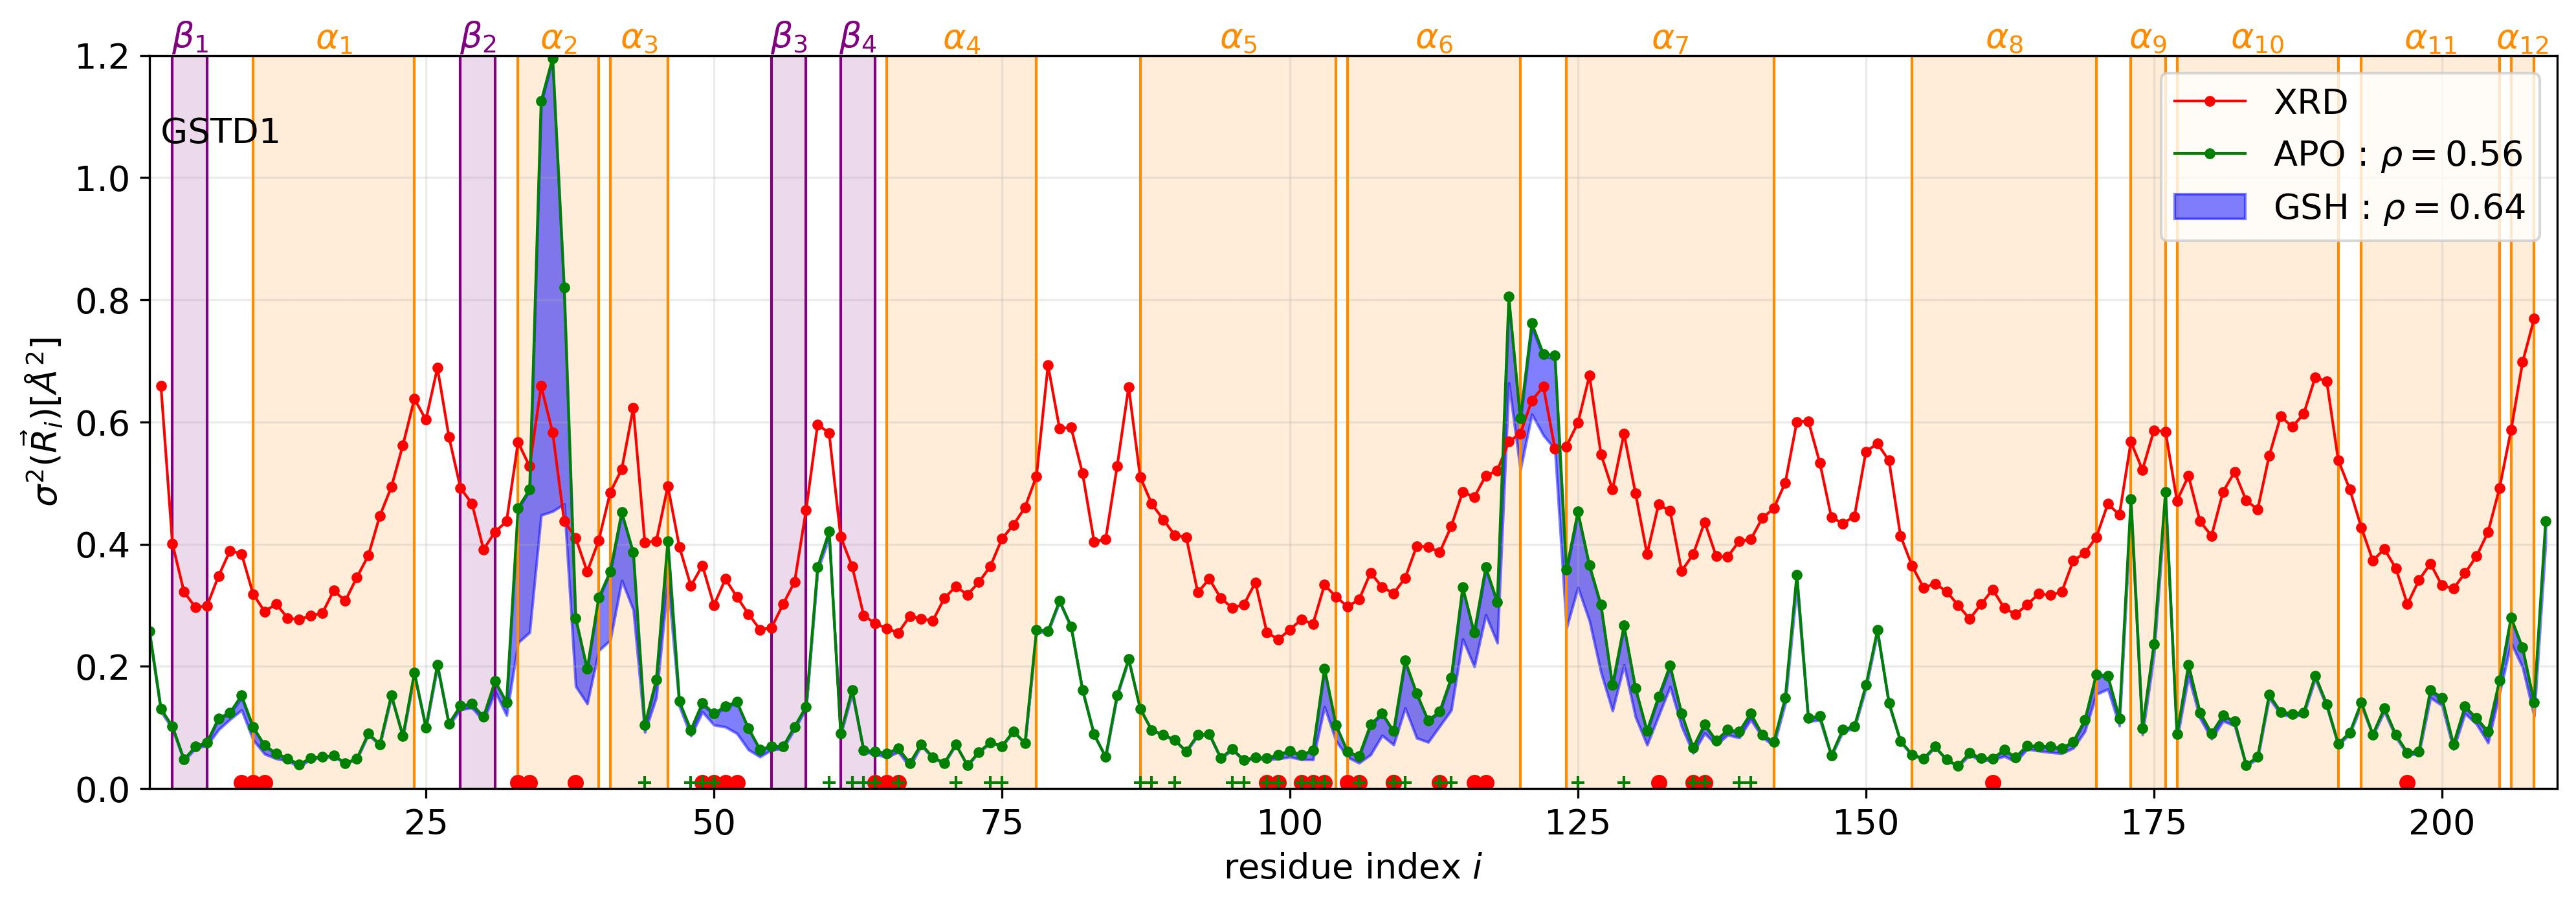
\includegraphics[width=\textwidth]{figures/GSTD1_APO+GSH_MSF.jpg}
	\end{minipage}
	\begin{minipage}{.49\linewidth}
		\textbf{(b)}\\
		
		\centering
		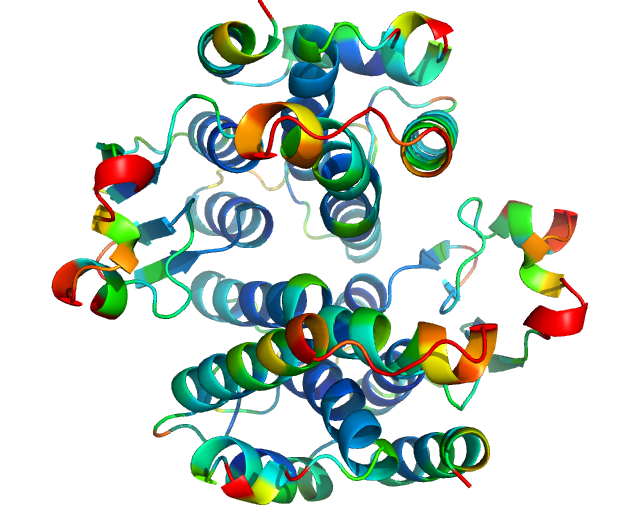
\includegraphics[width=.8\textwidth]{figures/GSTD1_APO_MSF.png}
	\end{minipage}
	\begin{minipage}{.49\linewidth}
		\textbf{(c)}\\
		
		\centering
		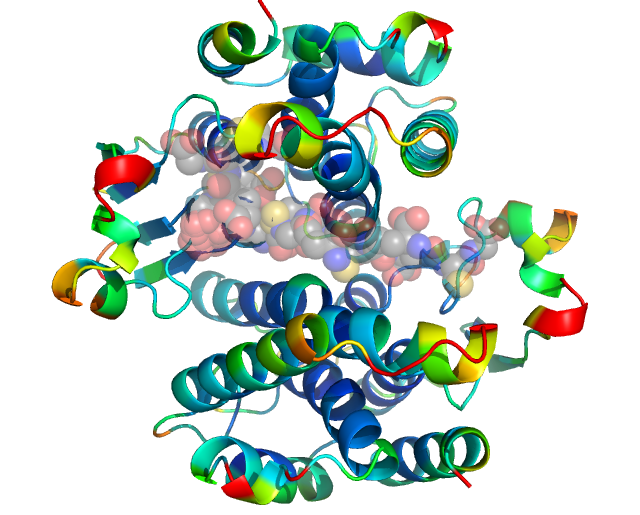
\includegraphics[width=.8\textwidth]{figures/GSTD1_GSH_MSF.png}
	\end{minipage}
	\caption{(a) Local Mean Square Fluctuations (MSF) predicted from ANM and comparison with experimental XRD data. Red and green points below represent the MAS index of amino acids belonging to the BSs and IoD, respectively. (b) Cartoon representation of the APO (unbound) GSTD1 structure. The color code corresponds to the local MSF range from 0 (blue) to 0.6~\AA$^2$ (red). (c) Cartoon representation of the GSH bound GSTD1 structure. The color code is the same as in panel b.}
	\label{Local MSF D1}
\end{figure}

Then, we compared the local MSF with the ones measured experimentally using XRD (add reference). We found that the comparison between ANM calculations and XRD data is overall in good agreement, with a Pearson correlation $\rho=0.56$ for APO and $\rho=0.64$ for the GSH bound structure of GSTD1. The main differences come from regions $33-52$ and $103-130$, as described above. In these two regions, the local flexibility predicted by ANM is slightly overestimated. However, it was even worse without the presence of the ligands, which confirms that the influence of the ligand is not negligible and should be taken into consideration for the prediction of the local flexibility of GSTs using ANM. Finally, regions $33-52$ and $103-130$ are located at the periphery of the protein surface. It means that these two regions are in interactions with solvent molecules when the protein is in its environment. The hypothesis here is that theses interactions will act as the ligand and decrease the flexibility of these two particular regions. Here, the interactions with solvent molecules are not taken into account since they are not predicted from AlphaFold. It is doable to add solvent molecules around the protein using programs such as Packmol (add reference, \bulurl{https://m3g.github.io/packmol/}). To test the hypothesis, we will include the first water shell of solvent molecule in the near future.\\

We performed the exact same ANM calculations for the 25 GST structures predicted from AlphaFold. Local MSFs as a function of MSA index are presented in Fig.~\ref{MSF + MSA}. \noindent From this map, we can identify regions of conserved high flexibility. First we identify that the N and C-terminal parts are much more flexible than the rest of the structure. Second we identify regions of high flexibility for MSA indices $j=40;  41;  42$. Computing the mean of MSF over all the different structures, we computed what we called region of conseved high flexibility. Taking values of MSF for gaps as $0.0$\AA , and considering only the MSA indices that have less than $15$ gaps, we selected an ensemble of MSA indices $j = 30;  40;  41;  42;  47;  66;  85;  86; 129; 132; 133; 135; 156; 185; 228; 234; 235; 236; 237; 238$.

\begin{figure}[h!]
	\textbf{(a)}\\
	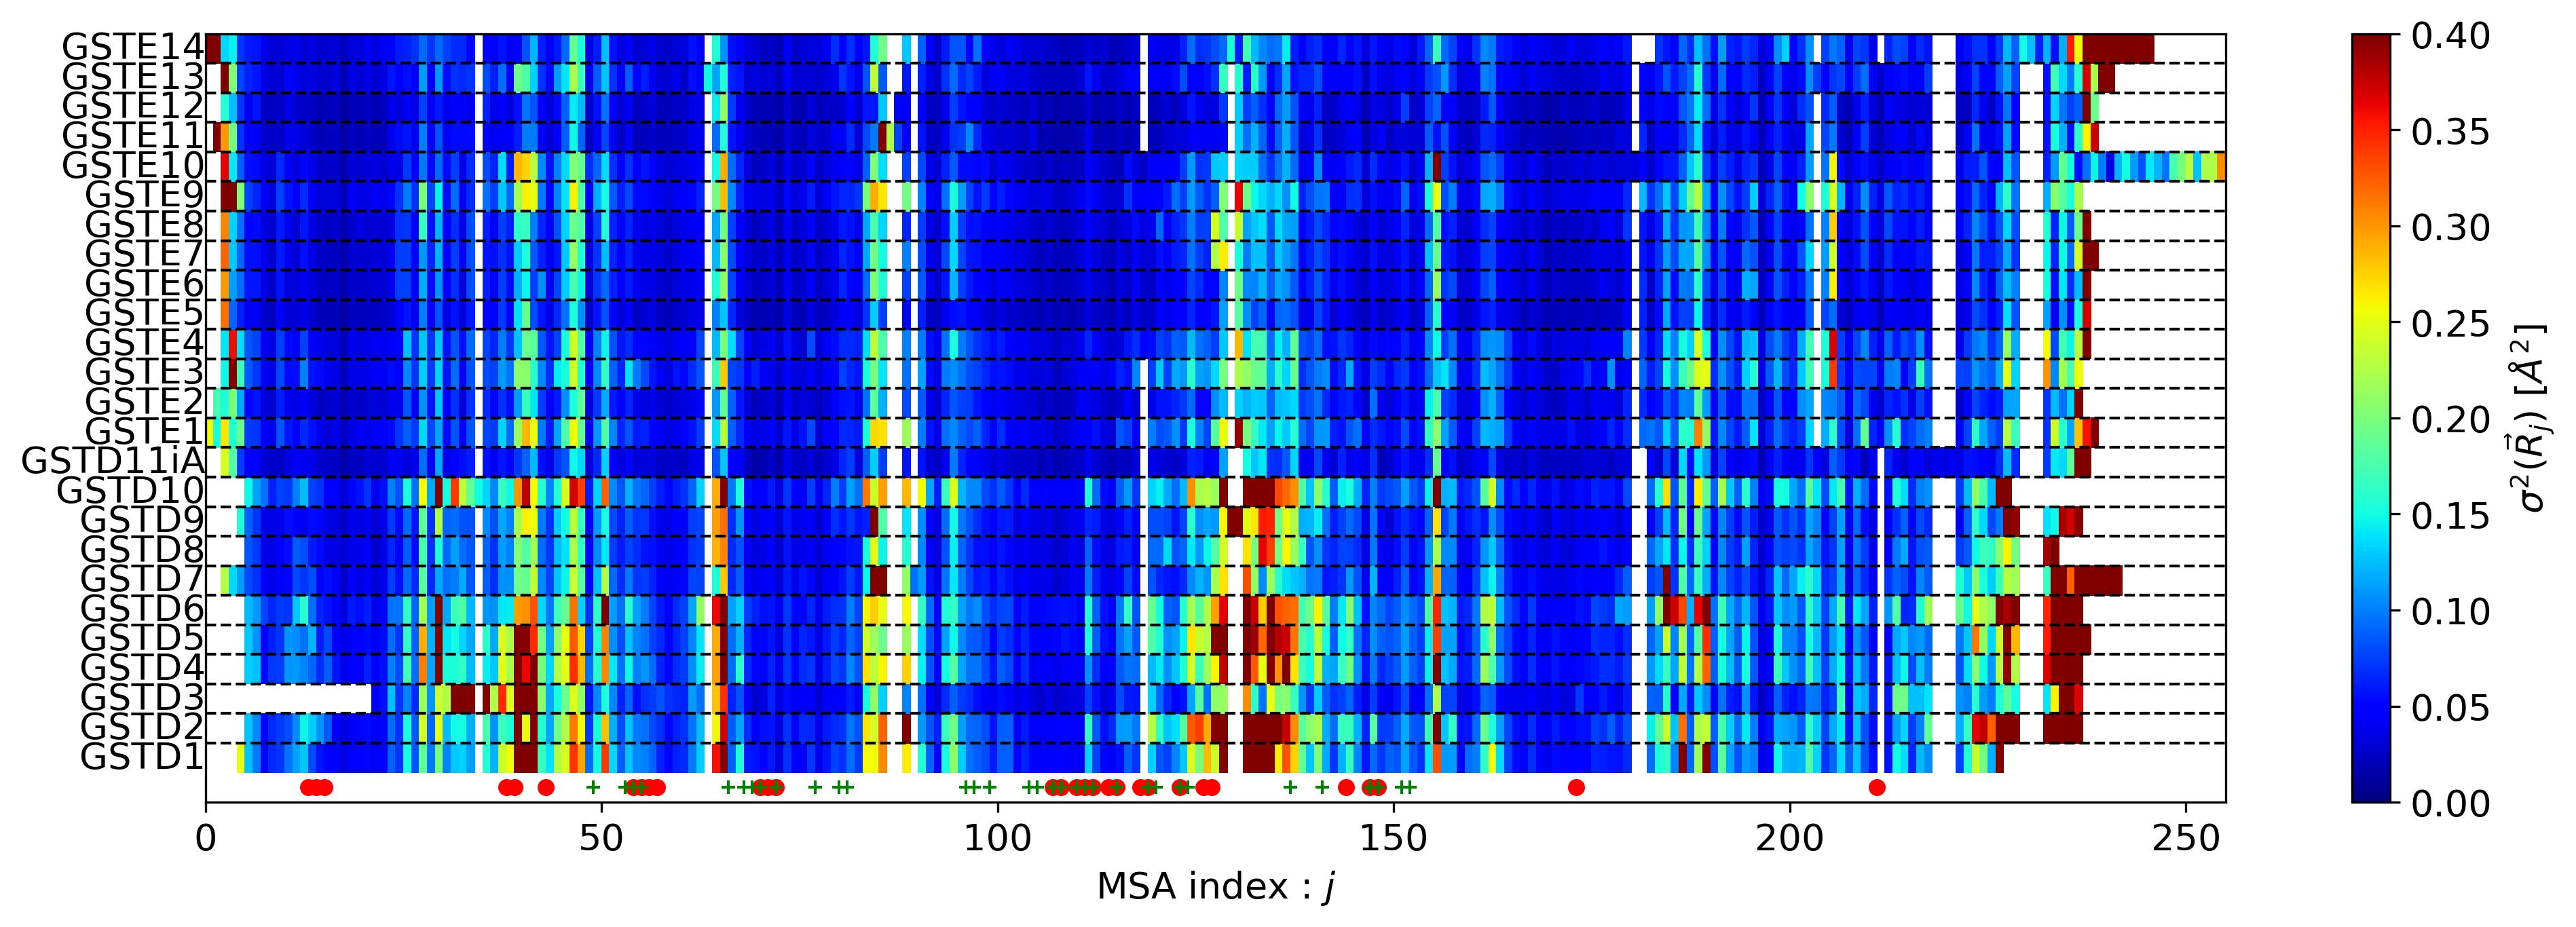
\includegraphics[width = .99\linewidth]{figures/ANM-COM+MSA_GSH_MSF.jpg}\\
	\textbf{(b)}\\
	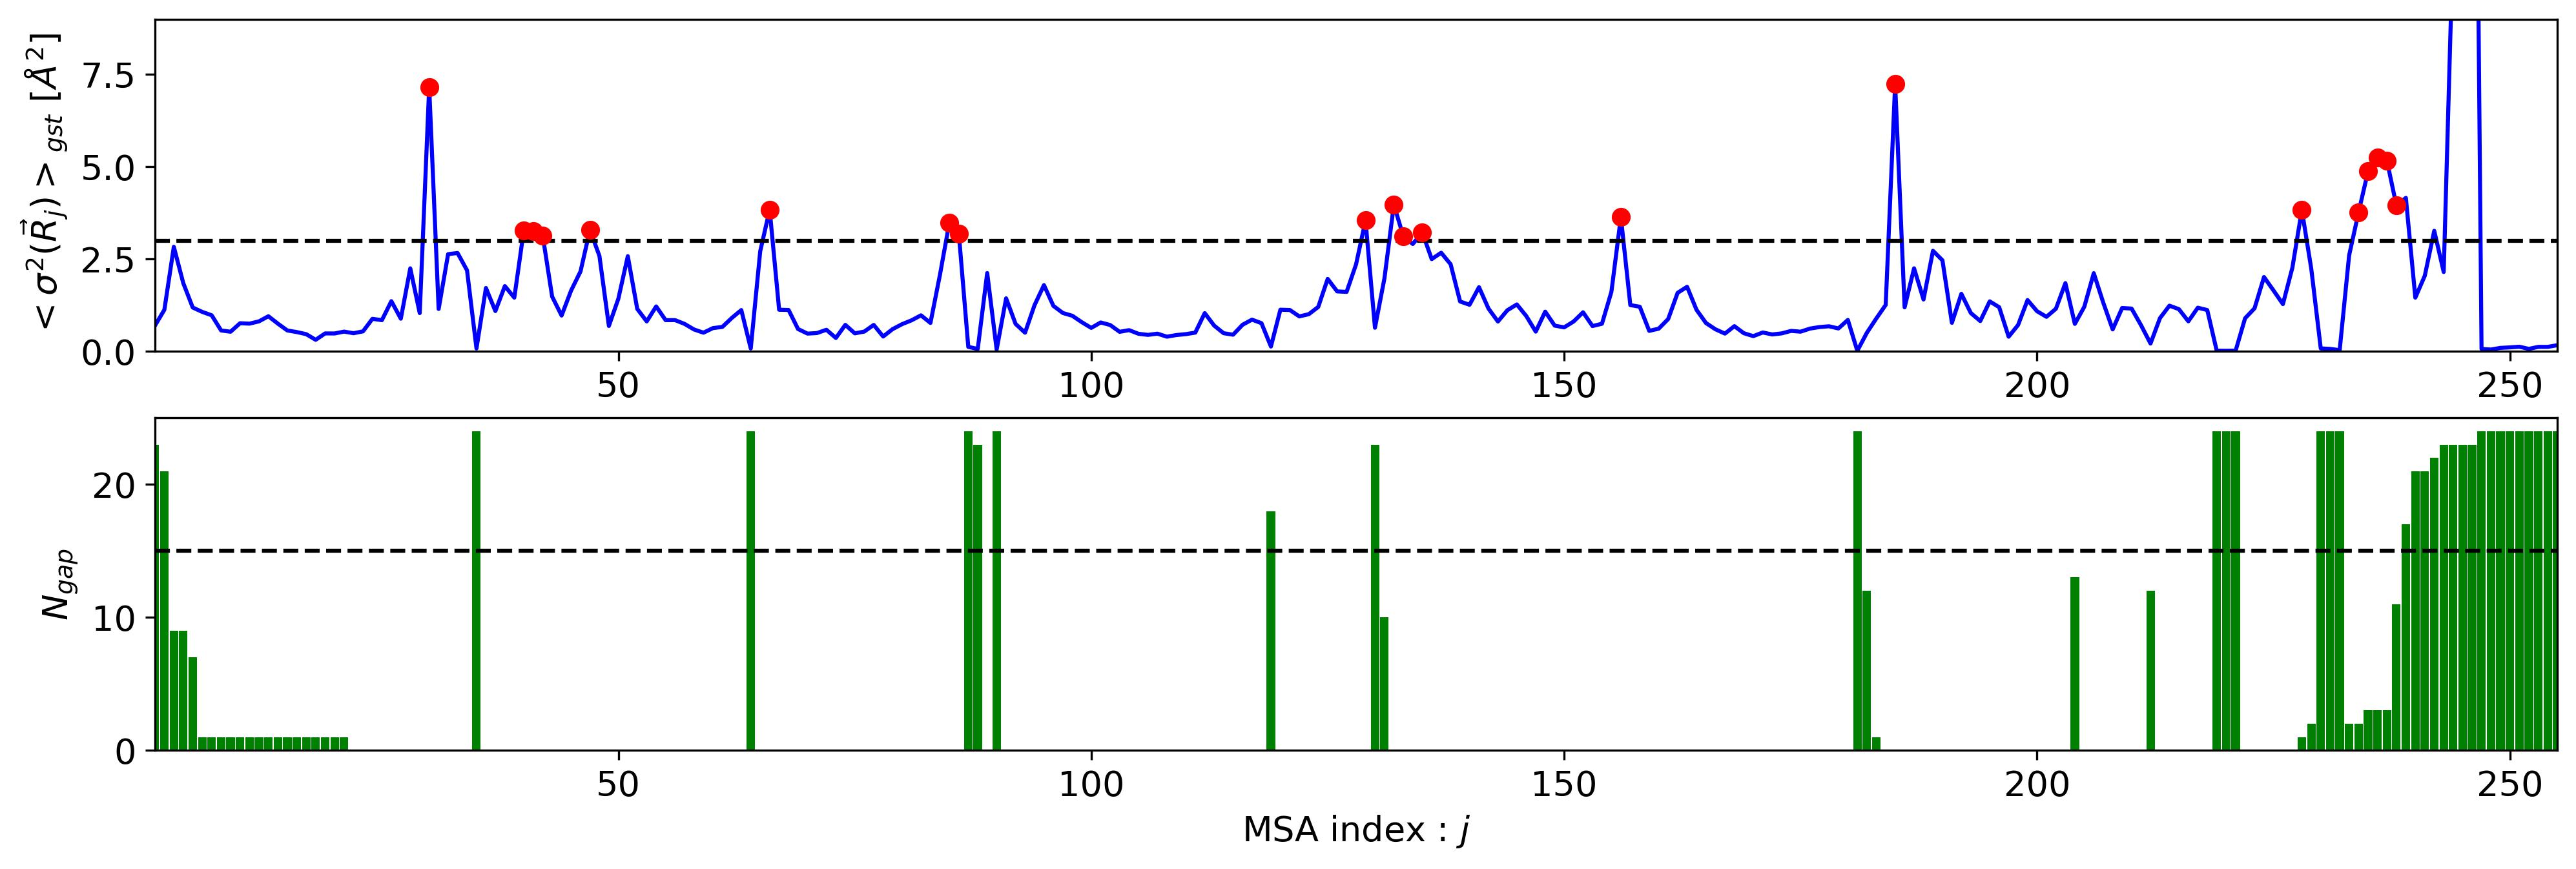
\includegraphics[width = 16cm]{figures/Local_MSF_key_residues.jpg}
	\caption{\textbf{(a)} Local MSF (in \AA$^2$) computed from ANM including GSH ligands as a function of the MSA index for the ensemble of 25 GSTs. Red and green points below represent the MAS index of amino acids belonging to the BSs and IoD, respectively.\textbf{(b)} Mean over computed local MSF for the ensemble of 25 GSTs. Red dots points the conserved highly flexible residues.}
	\label{MSF + MSA}
\end{figure}

\subsection{Non-Local Mean Square Fluctuations}

Figure \ref{Non-local MSF GSTD1} represents the non-local Mean Square Fluctuations (MSF) $\sigma^2 (\vv{R}_{ij})$ computed from Eq.(\ref{metric dij}) for the GSTD1 structure.  Compared to local MSF, non-local MSF correspond to the flexibility of a pair of amino acid $(i,j)$ in the sequence. As shown in X, particular patterns are observed in the non-local MSF matrix of the GSTD1, with lines being well defined corresponding to singular behavior of specific amino acids.

In GSTD1, we identified the pairs of amino-acid $30;122$ that corresponds to the intersections of two lines in this matrix. As shown in figure XXX, those lines appears in every computed $\sigma^2(\vv{R}_{ij})$. In order to identify conseved pairs, computed the mean matrix also taking into account gaps as null values. From this computed matrix, we identified pairs of MSA indices $()$... 

\begin{figure}
	\label{Non-local MSF GSTD1}
	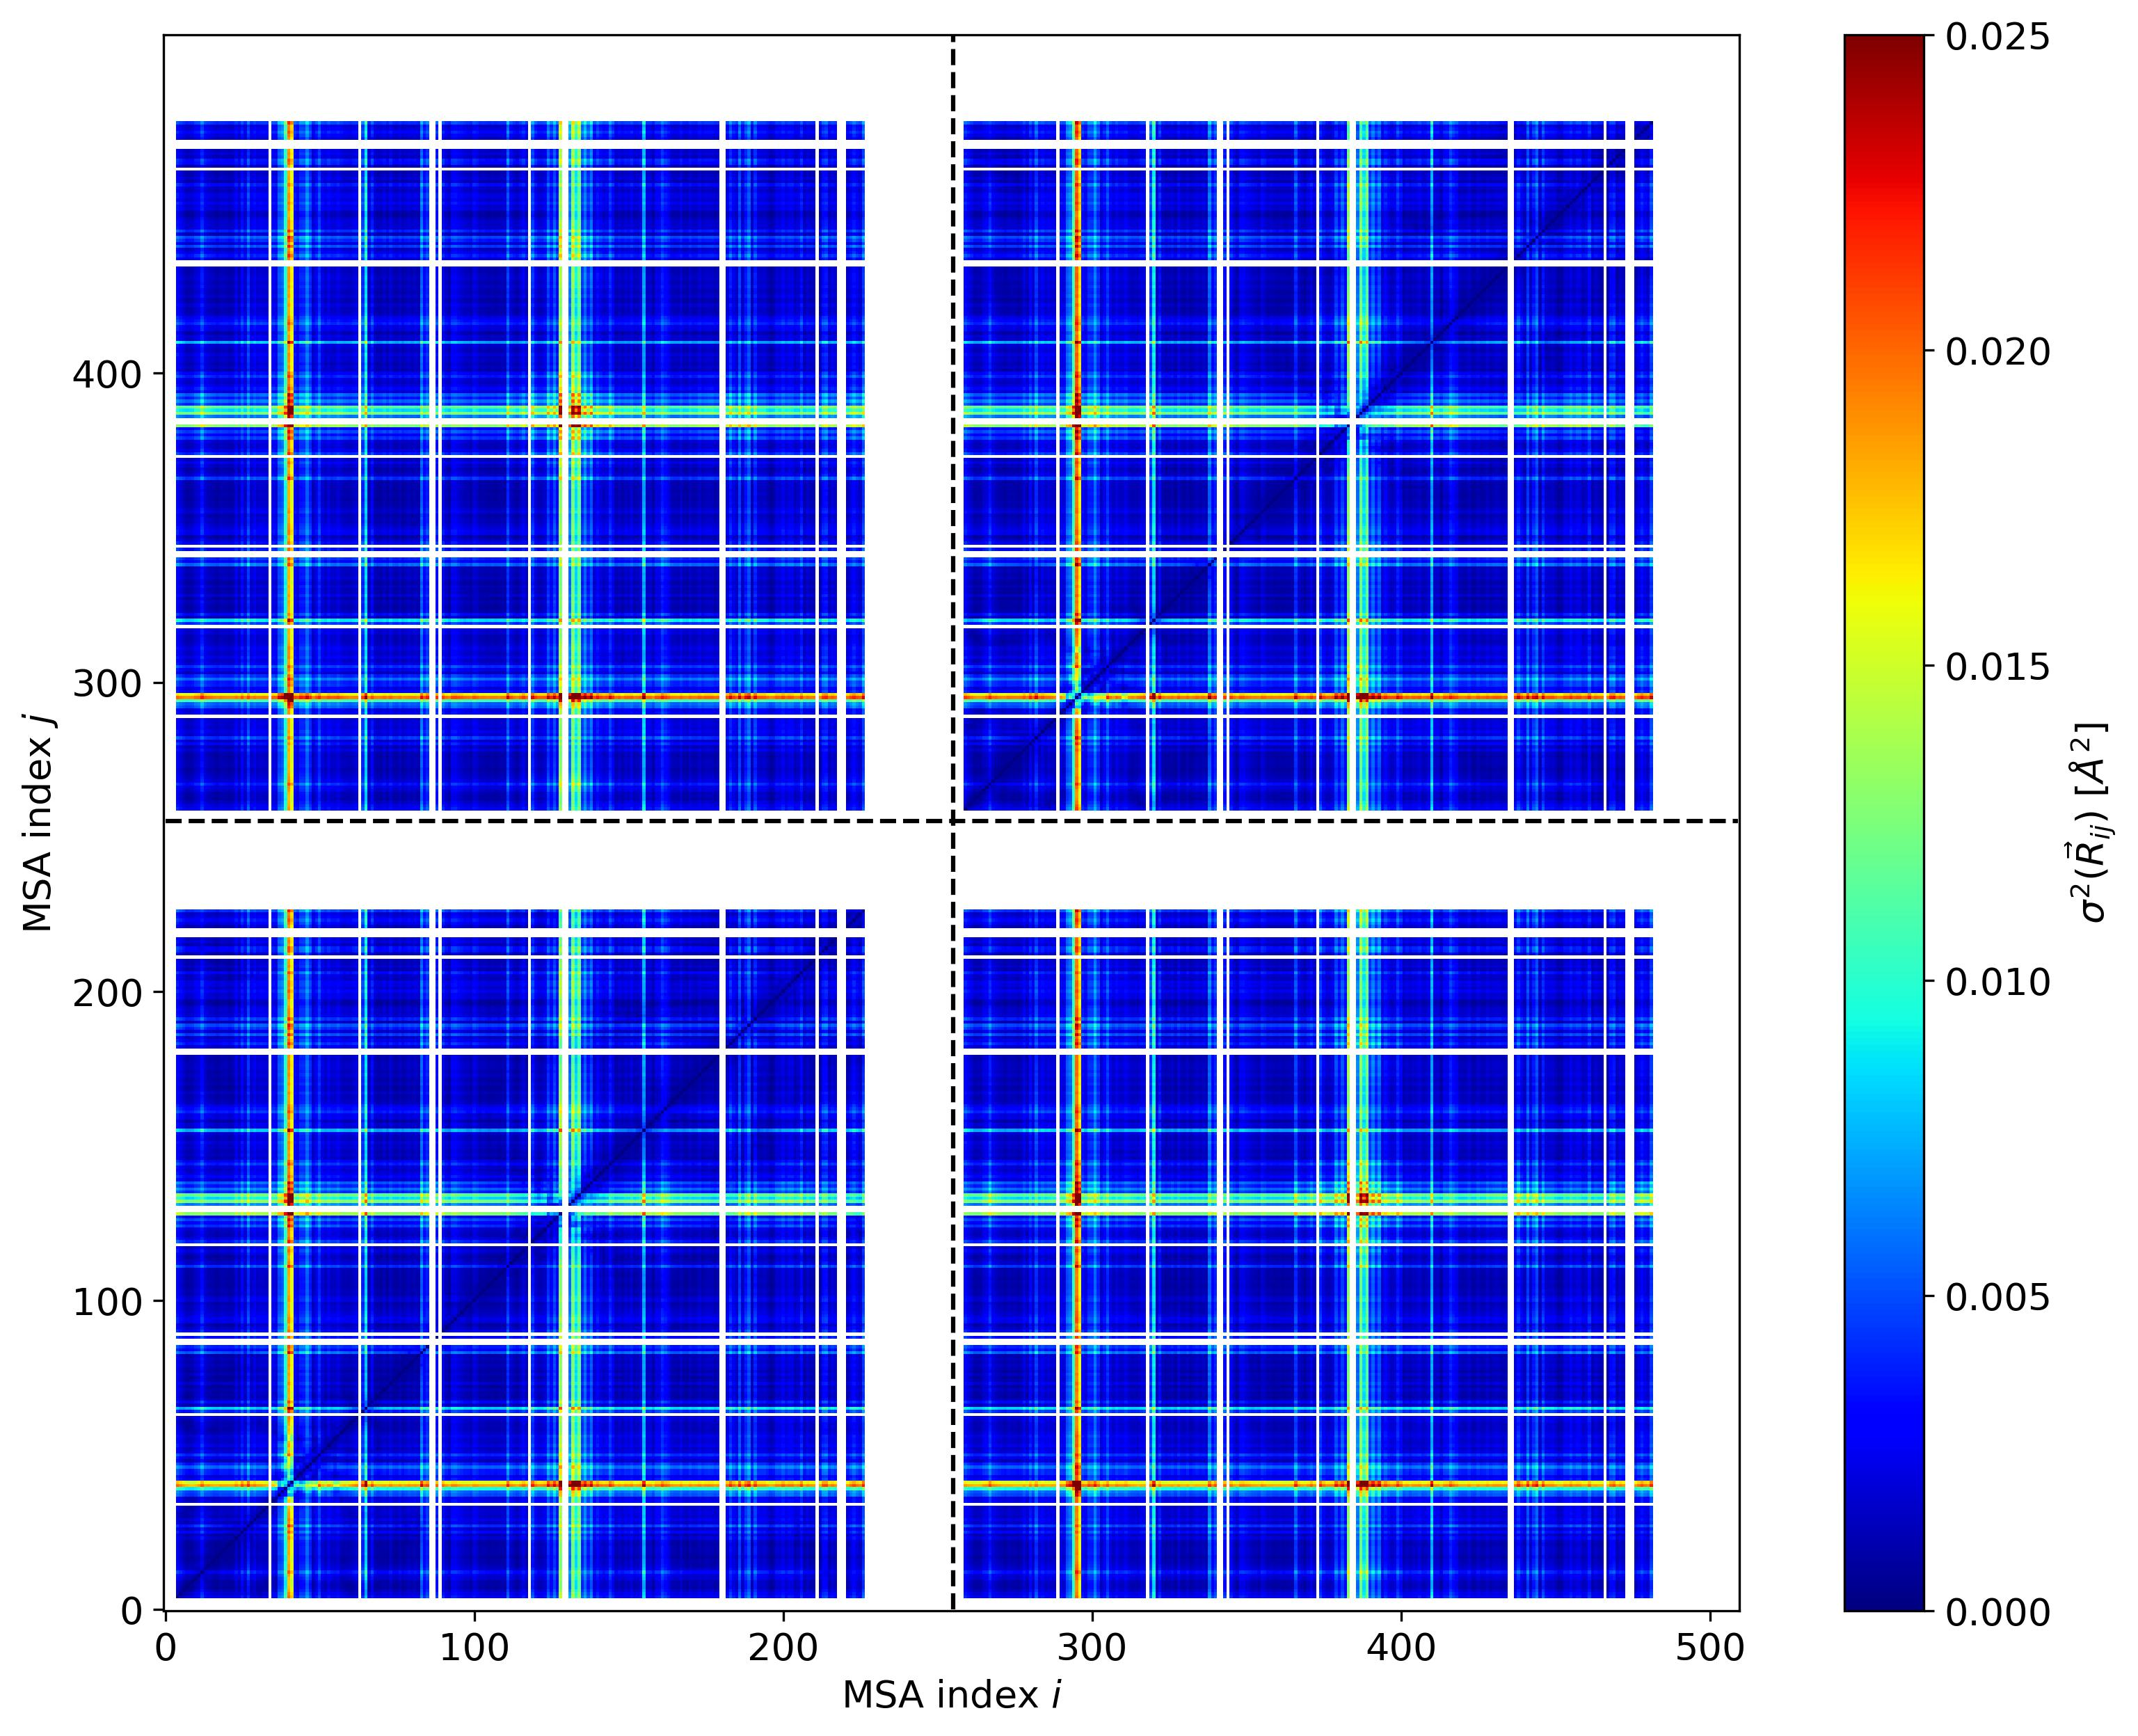
\includegraphics[width = 8cm]{figures/ANM-COM+MSA_GSTD1_APO_non-local_MSF}
	\caption{Non-local MSF matrix computed for the GSTD1 structure}
\end{figure}

\section{Identification of conserved key residues}

From the computed local and non-local thermal MSF, we identified regions of high flexibility. From figure \ref{MSF + MSA}, we computed the mean local MSF as a function of the MSA index. It allowed to identify what we called conserved high flexibility. We identified the MSA indices presented in the table bellow. In the case of GSTD1, we computed the non-local MSF and extracted the MSA indices presented bellow. We are currently working on a way to extract pairs conserved residues from the 25 different structures of GSTs.

\begin{table}[h!]
	\begin{tabular}{cp{4cm}p{5cm}p{4.5cm}}
		\hline
		\hline
		& High conservation & Medium conservation & Low conservation \\
		\hline
		\multirow{2}{*}{Local MSF} & •   $3$ & •  $30$ & • $33$ \\
		                           & • $190$ & •  $32$ & • $36$ \\
		                           &         & •  $34$ & • $40$ \\
		                           &         & •  $41$ & • $129$ \\
		                           &         & •  $42$ & • $132$ \\
		                           &         & •  $85$ & • $135$ \\
		                           &         & • $130$ & • $185$ \\
		                           &         & • $131$ & • $233$ \\
		                           &         & • $133$ & • $235$ \\
		                           &         & • $134$ & • $236$ \\
		                           &         & • $156$ & • $237$ \\
		                           &         & • $228$\\
		                           &         & • $229$\\
		\hline
		\multirow{2}{*}{Non-local MSF} & • $23$ & • $41$ & • $135$ \\
		                               & • resi & • $133$ &  \\
		\hline
		\hline
	\end{tabular}
	\caption{Identification of conserved key residues}
	\label{Final table}
\end{table}
